\documentclass{manual}
\pagenumbering{gobble}

\usepackage{listings}

\title{MQTT CO2 Sensor}
\author{Blaise J Thompson}

\begin{document}

\maketitle

\vspace*{\fill}

\includegraphics[width=\textwidth]{"../photos/IMG_7934"}

\vspace*{\fill}


\section{Description}
\pagenumbering{arabic}

This manual documents the construction and development of the wireless, distributed CO2 sensor project.
These WiFi-enabled sensors broadcast data via \href{https://mqtt.org/}{MQTT}.

\section{Wiring}

\subsection{Bill of Materials}

\begin{itemize}
  \item CO2 sensor (CO2METER.COM K30 - \$85)
  \item microcontroller (Adafruit ``Huzzah'' 2471 - \$10)
  \item 5 V regulator (Pololu 2843 - \$5)
  \item barrel jack (Switchcraft 722A - \$2)
  \item 2x 4.7k$\Omega$, 0.25 W resistors
  \item barrel jack holder, polycarbonate mounting plate (homemade)
\end{itemize}

\subsection{Wiring}

Wiring is pretty simple, you can see all of it here.
Note that the two pull-up resistors are underneith the micro-controller.
The HUZZAH break-out board has awkwardly small mounting holes, so we ended up using M2 screws.

\includegraphics[width=\textwidth]{"../photos/IMG_20200630_155026.jpg"}

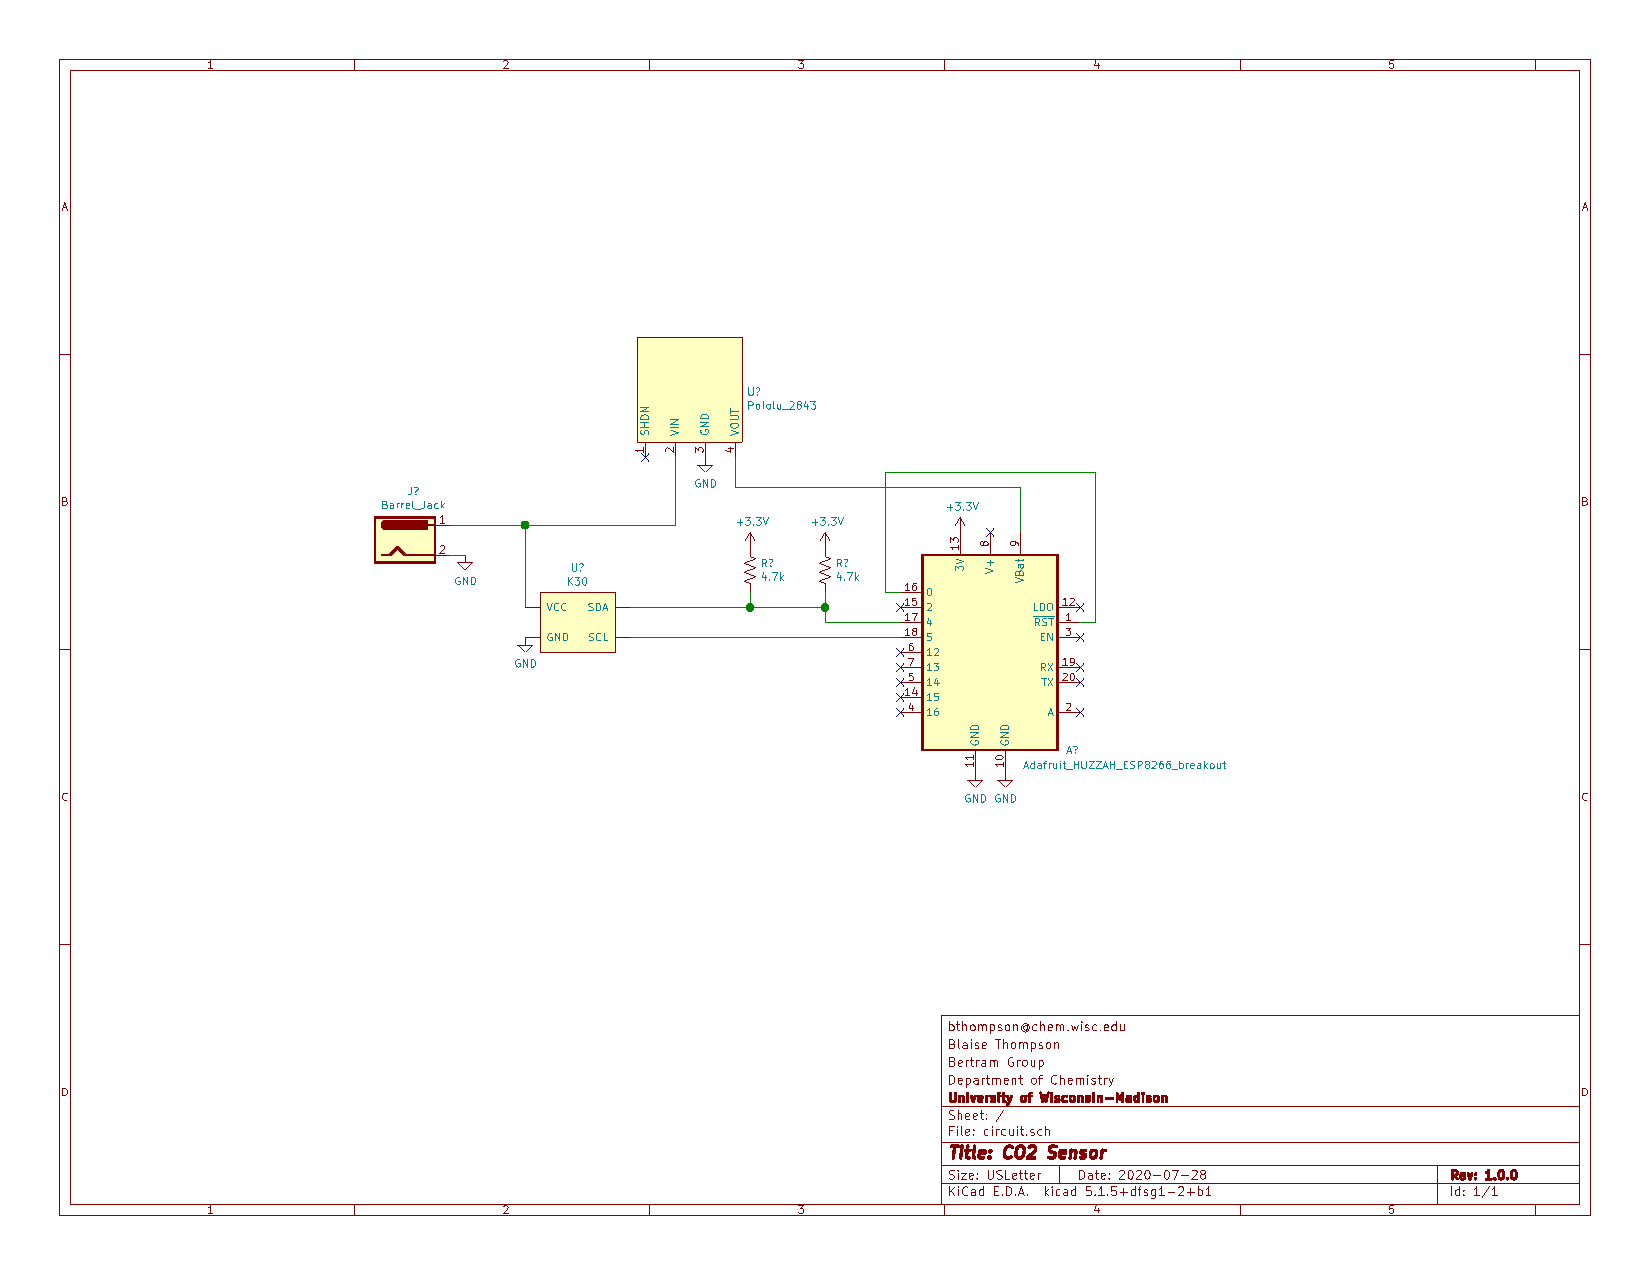
\includepdf[landscape=true]{../circuit/circuit.pdf}

\subsection{Power Considerations}

9-14 V input power (2.1 mm barrel, center positive).

32 hours battery life with 6 AA.

\section{Firmware}

This section describes the firmware that was flashed to the ESP8266 microcontroller.
This project was built on-top of the open-source microhomie firmware, in particular microhomie-esp8266-v2.4.0-beta1. \\
The pre-compiled binary can be downloaded from GitHub: \\
\url{https://github.com/microhomie/microhomie/releases/tag/v3.0.0-beta1}.

\subsection{main}

main.py is automatically run by micropython when the controller initializes.
In this case, we create a single HomieDevice and run it forever.
Note that microhomie uses uasyncio to enable async-await syntax in micropython.

\includepython{../firmware/main.py}

\clearpage
\subsection{settings}

microhomie automatically reads configuration details from a file called ``settings.py''.
Some values have been redacted as, unfortunately, login credentials for the private network cannot be shared.

\includepython{../firmware/settings.redacted.py}

\subsection{flash}

The following bash script was used to flash the microcontroller.
Importantly, the ID field must be changed for each device before flashing.
This flash script uses \href{https://github.com/espressif/esptool}{esptool} and \href{https://github.com/scientifichackers/ampy}{ampy}, both python utilities.
Blaise also recommends \href{https://github.com/dhylands/rshell}{rshell} for debugging the microcontroller, including remote REPL and incremental file transfer.

\includebash{../firmware/flash.sh}

\section{Server}

These devices are, of course, able to publish to any MQTT broker as configured in firmware.
In this case, they have been programmed to publish to \url{https://mqtt.chem.wisc.edu}.
This server also runs a database application with a little bit of custom Python to link things together.
All of this runs using Docker.
See the git repository at \url{https://git.chem.wisc.edu/infrastructure/mqtt} for complete documentation of how this server is put together.

You may interact with the server in several different ways.
These are documented on the website.

\end{document}
